\chapter{Refactoring}
\label{ch:refactoring}
El refactoring del c\'odigo original se realiz\'o en Python 3.6. Adem\'as se mantuvieron casi la totalidad de las librer\'ias cambiando \'unicamente Pymorph por Mahotas, debido a que la primera dej\'o de ser mantenida desde el 2010 y la segunda corresponde a la librer\'ia para Python 3.   

\section{Manejo de la rutina: \textsc{RoutineHandler}}

La \textbf{rutina} comprende el proceso de listado de archivos (que en esta nueva versi\'on se realiza en la clase \textsc{DataPicker}); los procesos iterativos de c\'alculo de flujo, obtenci\'on de estimaciones y la detecci\'on de candidatos con \textsc{SourceFinder}; y el guardado de la informaci\'on de los  candidatos y/o la generaci\'on de visualizaciones (dependiendo del tipo de ejecuci\'on). Estos procesos son administrados por la clase \textsc{RoutineHandler} el cual debe instanciarse recibiendo tres archivos descritos a continuaci\'on:


\begin{itemize}
\item Lista de campos, CCDs, semestres y, alternativamente, las coordenadas de alg\'un objeto de inter\'es, en un archivo CSV (en este mismo orden), teniendo como encabezado \texttt{Field, CCD, Semester, POS\_Y, POS\_X}. En caso de no adjuntar las coordenadas en los campos de posici\'on, se puede rellenar con un gui\'on (`-'). En el constructor este archivo se recibe como \texttt{obs\_index\_path} (ejemplo en Ap\'endice \ref{subs:sn_list}).
\item Diccionario de directorios y expresiones regulares de las ubicaciones de los archivos y sus nombres, respectivamente (archivo de formato CSV). En el constructor de la clase este archivo se denomina como \texttt{routes\_templates} (ejemplo en Ap\'endice \ref{subs:a1}).
\item Diccionario de umbrales y par\'ametros relevantes en la ejecuci\'on del programa, as\'i como el tipo de filtro a usar (archivo de formato CSV). En el constructor se denomin\'o \texttt{settings\_file} (ver ejemplo en Ap\'endice \ref{subs:settings_file}).
\end{itemize}
\bigskip

Adem\'as de estos archivos se debe especificar el \'indice de la fila a procesar de la lista de campos, CCDs y semestre (primer archivo de entrada). Esto se hizo as\'i con la finalidad de facilitar la paralelizaci\'on de los an\'alisis de diferentes conjuntos de datos. Por lo tanto el constructor de \textsc{RoutineHandler} queda como sigue:

\begin{center}
\texttt{RoutineHandler(obs\_index\_path, routes\_templates, settings\_file, index)}
\end{center}

El m\'etodo m\'as importante de esta clase es \texttt{routine}, el cual implementa la pipeline principal del programa orignal. Este m\'etodo puede ser ejecutado de dos formas, dependiendo de la finalidad que busca el usuario: si se desea realizar una b\'usqueda de candidatos (considerando tambi\'en las coordenadas entregadas en \texttt{obs\_index\_path}) o, si se desea visualizar informaci\'on de candidatos ya encontrados (a partir de una lista de coordenadas cargadas desde un archivo NPZ). La Figura \ref{fig:new_routine} muestra ambas formas de ejecuci\'on. La lista completa de m\'etodos de esta clase se encuentran en el Ap\'endice, secci\'on \ref{subs:a4}.

\begin{figure}
\centering
    \subfloat[B\'usqueda de candidatos]{{\includegraphics[scale=.5]{/home/paloma/Documents/Memoria/Code/sif2/sif2_act} }}%
    \qquad
    \subfloat[Generaci\'on de visualizaciones]{{\includegraphics[scale=.5]{/home/paloma/Documents/Memoria/Code/sif2/sif2_act2} }}%
\caption{Rutina del programa refactorizado. Cuenta con dos modos de ejecuci\'on: uno de b\'usqueda de candidatos (izquierda) y otro de generaci\'on de gr\'aficos (derecha). Pueden ejecutarse ambas formas comenzando con la b\'usqueda de candidatos y continuar con el modo de generaci\'on de gr\'aficos. El usuario tiene la libertad de escoger el modo de ejecuci\'on.}
\label{fig:new_routine}
\end{figure}  
%\section{Ejecuci\'on de la rutina}
\section{Manejo de datos de entrada}
Todas las im\'agenes de entrada son manipuladas y servidas por la clase \textsc{DataPicker}. Esta clase se inicializa recibiendo un \textit{path} hacia el archivo de configuraci\'on \texttt{routes\_templates} que contiene tanto las rutas a los archivos as\'i como los nombres de estos en t\'erminos de expresiones regulares; semestre a los que corresponde la secuencia de observaciones (los dos \'ultimos d\'igitos del a\~no concatenados con la letra A en caso de corresponder al primer semestre o B al segundo); el campo (representado como un n\'umero de dos d\'igitos, comenzando con cero para valores menores a 10) y el detector CCD (cadena de tres car\'acteres donde el primero de ellos describe a que grupo de detectores corresponde: N o S (ver Figura \ref{fig:f4}); adem\'as de un n\'umero entero que va de 1 a 36) como strings (para m\'as detalles, ver Ap\'endice, secci\'on \ref{subs:des_rutas}). 
\bigskip

Es en \textsc{DataPicker} donde se realiza el proceso de filtrado de las im\'agenes (descarte por \gls{airmass}) y su posterior ordenamiento, esta vez considerando un filtrado m\'as minucioso, considerando la correspondencia de las fechas MJD contenidas en los header de cada archivo FITS. Para ver los detalles de este proceso de listado de im\'agenes y filtrado, revisar el Ap\'endice, secci\'on \ref{subs:a2}.

\section{Determinaci\'on de flujos}
El c\'alculo del flujo, en este refactoring, se independiz\'o del manejo de archivos (en el programa original estaba alojado en la clase \textsc{FITSHandler}) y se implement\'o en el script \texttt{utils} pensado como librer\'ia (una descripci\'on detallada de los m\'etodos se encuentra en el Ap\'endice, secci\'on \ref{ap:utils}).
\bigskip

\section{Filtros originales}
La refactorizaci\'on de los filtros de Kalman originales implic\'o la implementaci\'on de nuevas clases e interfaces para el desarrollo del patr\'on propuesto: Strategy (ver familia de m\'etodos resultante en la Figura \ref{fig:ref1}). A continuaci\'on se presentan cada una de ellas:

\begin{itemize}
\item \textbf{IPredict:} Interface que describe el comportamiento de la funci\'on \textsc{Predict} de un filtro de Kalman. El m\'etodo \texttt{predict} recibe como par\'ametros el paso de tiempo ($\Delta t$), la matriz de estado, la matriz de covarianza de estado, y las predicciones de las matrices de estado y covarianza determinadas en el paso anterior (con la finalidad de actualizar estas variables). Su firma queda como:
\begin{center}
\texttt{predict(delta\_t, state, state\_cov, pred\_state, pred\_cov)}
\end{center}
Este m\'etodo entrega finalmente las matrices de estado y covarianza de estado predicho.
\bigskip

\item \textbf{ICorrect:} Interface que describe el comportamiento de la funci\'on \textsc{Correct} de un filtro de Kalman. El m\'etodo \texttt{correct} recibe como par\'ametros la matriz de flujo (\texttt{z}, correspondiente a la observaci\'on) y de varianza de la observaci\'on (\texttt{R}), las matrices de estado y covarianza predichas y las matrices de estado y covarianza estimadas obtenidas en el paso anterior y que ser\'an actualizadas. Su firma queda como:
\begin{center}
\texttt{correct(z, R, pred\_state, pred\_cov, state, state\_cov)}
\end{center}
\bigskip
Esta funci\'on entrega finalmente las matrices de estado y covarianza de estado corregido.

\end{itemize}

\subsection{Predicci\'on}
\textbf{LinearPredict:} Clase que extiende IPredict. Implementa el m\'etodo \texttt{predict} que ser\'a usado tanto por el filtro b\'asico como por el de m\'axima correntrop\'ia. Su instanciaci\'on recibe como argumento \texttt{sigma\_a} (desviaci\'on est\'andar del ruido del proceso, asumiendo una distribui\'on gaussiana para las observaciones).
\bigskip


\subsection{Correcci\'on}
\textbf{BasicCorrect:} Clase que extiende ICorrect. Implementa el m\'etodo \texttt{correct} que ser\'a usado para el tipo de filtro de Kalman b\'asico.
\bigskip

\textbf{MCCorrect:} Clase que extiende ICorrect. Implementa el m\'etodo \texttt{correct} que ser\'a usado para el tipo de filtro de Kalman de m\'axima correntrop\'ia. El constructor de esta clase recibe los siguientes par\'ametros:

\begin{itemize}
\item \texttt{epsilon}: Cantidad con la cual se contrastar\'a el error o precisi\'on que se quiera lograr con la estimaci\'on (el valor definido por defecto en el programa original es de $10^{-6}$).
\item \texttt{max\_iter}: N\'umero m\'aximo de iteraciones (de acuerdo al c\'odigo orignal, se estableci\'o como $10$ su valor por defecto).
\item \texttt{silverman}: \textit{boolean}. Determina si se usa o no la apoximaci\'on de Silverman para el ancho de banda del kernel Gaussiano (por defect es \textit{false}).
\item \texttt{std\_factor}: Factor de desviaci\'on est\'andar usado en la aproximaci\'on de Silverman (su valor predeterminado es de $100,0$).
\item \texttt{sigma}: Sigma usado para el ancho de banda en el c\'alculo de la correntrop\'ia. Puede ser o no optimizado por Silverman. Por defecto, es $1000,0$, seg\'un programa original.
\end{itemize}

\subsection{Filtros refactorizados}

\begin{itemize}
\item \textbf{KalmanFilter:} Clase abstracta padre de los subtipos BasicKalmanFilter y MCKalmanFilter. Posee los m\'etodos abstractos \texttt{predict} y \texttt{correct}, que son definidos de acuerdo a las estrategias de predicci\'on y correci\'on descritas previamente.
\item \textbf{BasicKalmanFilter:} Representa el filtro b\'asico de Kalman. Est\'a compuesto por las estrategias \texttt{LinearPredict} y \texttt{BasicCorrect}.
\item \textbf{MCKalmanFilter:} Representa el filtro de m\'axima correntrop\'ia. Est\'a compuesto por las estrategias \texttt{LinearPredict} y \texttt{MCCorrect}.
\end{itemize}
\bigskip

\begin{figure}
\centering
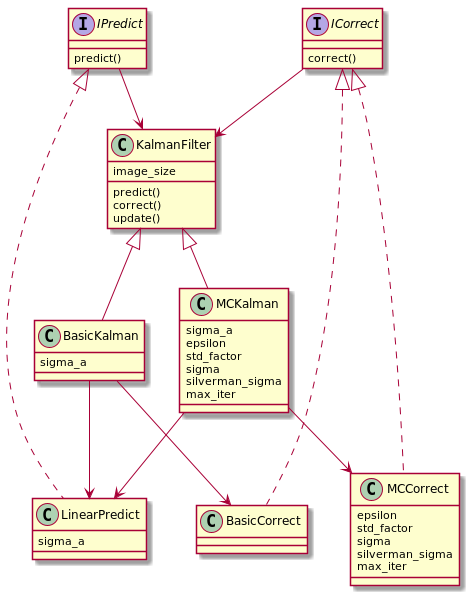
\includegraphics[scale=.5]{images/kalmanfilter_class}
\caption{Familia de filtros de Kalman y patr\'on \textit{strategy} usado en la implementaci\'on de los m\'etodos \texttt{predict} y \texttt{correct}.}
\label{fig:ref1}
\end{figure}

\section{Detecci\'on de candidatos}
\label{sec:detec}
Mientras que la detecci\'on de candidatos en el programa original se realiza en una instancia de la clase \textsc{SNDetector}, la detecci\'on en la nueva versi\'on se realiza en \textsc{SourceFinder}, el cual funciona de la misma forma que su antecesor. El cambio de nombre representa la intencionalidad de extender la funcionalidad de esta clase no s\'olo a la detecci\'on de supernovas sino adem\'as encontrar objetos como estrellas variables.
\bigskip

Su constructor requiere los siguientes argumentos:
\begin{itemize}
\item \texttt{flux\_thresh:} Umbral de corte para el flujo estimado por el filtro de Kalman.
\item \texttt{flux\_rate\_thresh:} Umbral de corte de velocidad de flujo estimado por el filtro de Kalman.
\item \texttt{rate\_satu:} Tasa de saturaci\'on en la velocidad de flujo.
\item \texttt{accum\_neg\_flux\_depth:} Cantidad de \'epocas de registro de p\'ixeles negativos (para la construcci\'on de una matriz de \textit{booleans} de esta profundidad).
\item \texttt{accum\_med\_flux\_depth:} Cantidad de \'epocas de registro de p\'ixeles cuya intensidad mediana (durante las \'epocas) es mayor a 1500.
\item \texttt{image\_size:} Dimensi\'on de las im\'agenes FITS (por defecto, corresponde a la tupla (4094, 2046)).
\item \texttt{n\_consecutive\_obs:} N\'umero de alertas u observaciones consecutivas a considerar para confirmar una detecci\'on. Para las versiones antigua y nueva de este programa, se estableci\'o como $4$.

\end{itemize}

Los m\'etodos se encuentran descritos en el Ap\'endice, secci\'on \ref{ap:sourcefinder}. Adem\'as, cabe mencionar que los par\'ametros previamente mencionados se ajustan al archivo de configuraci\'on, \texttt{settings\_file}.


\section{Visualizaci\'on de resultados}
En el proceso de visualizaci\'on participan dos clases: \textsc{Observer} y \textsc{Visualizer}. La primera clase es la encargada de generar una lista de diccionarios dentro de los cuales se almacena informaci\'on de los candidatos encontrados durante el proceso de detecci\'on. Esta lista es guardada como una variable de instancia en \textsc{Observer} denominada \texttt{objects} y la informaci\'on contenida por cada uno de los diccionarios corresponde a las siguientes componentes:

\begin{itemize}
\item Ubicaci\'on del objeto en la primera imagen cient\'ifica procesada, como un arreglo de \textit{floats} de largo dos. 
\item Lista de \'epocas en las que el objeto fue detectado.
\item Listas de estampillas de diferente profundidad, de ancho y alto $21 \times 21$. Las estampillas de cada lista tendr\'an una profundidad propia dependiendo desde la estructura que se extraigan. Estas estructuras pueden ser im\'agenes como la cient\'ifica, de diferencia, m\'ascara, etc., o a estructuras como las etiquetas de p\'ixeles grupales e individuales, matrices de estado, etc. Cada una de las estampillas de cada lista corresponder\'a a la medici\'on, c\'alculo o estimaci\'on obtenida para una \'epoca espec\'ifica. Adem\'as cada una de las estampillas est\'a centrada en la coordenada del objeto candidato a revisar.   
\end{itemize}
\bigskip

Para el registro de estos datos se emplean dos m\'etodos de \textsc{Observer} listados a continuaci\'on:

\begin{itemize}
\item \texttt{set\_space (cand\_data):}\\
Recibe lista de candidatos (coordenadas) \texttt{cand\_data} y crea lista de diccionarios, \texttt{objects}, con la finalidad de guardar la informaci\'on de los primeros para todas las \'epocas analizadas creando arreglos (de la librer\'ia \textsc{Numpy}) de estampillas $21 \times 21$ destinadas a guardar los datos de las diferentes estructuras: im\'agenes, matrices de estado estimado y predicho, covarianzas por pixel, matrices de etiquetas de p\'ixeles, etc. Cada estampilla estar\'a centrada en la posici\'on del candidato en la primera imagen cient\'ifica analizada. 
\bigskip

\item \texttt{look\_candData(cand\_data, pred\_state, pred\_state\_cov, kalman\_gain, state, state\_cov, time\_mjd, flux, var\_flux, science, diff, psf, base\_mask, dil\_base\_mask, pixel\_flags, pixel\_group\_flags, mjd\_idx):}\\
Con el espacio generado en la estructura \texttt{objects}, se procede a ejecutar la pipeline principal (c\'alculo de flujo, generaci\'on de estimaciones con filtro de Kalman y proceso de detecci\'on) para, en esta ocasi\'on, ir guardando resultados de los candidatos en \texttt{cand\_data} en su diccionario respectivo por cada \'epoca (cuyo \'indice est\'a representado por el argumento \texttt{mjd\_idx}). Por tanto recibe como argumentos las matrices de estados y covarianzas predichos (\texttt{pred\_state} y \texttt{pred\_state\_cov} respectivamente), las matrices de estados y covarianzas estimados (\texttt{state} y \texttt{state\_cov}) la matriz de ganancia de Kalman (\texttt{kalman\_gain}), matriz de flujo calculado y varianza asociada (\texttt{flux} y \texttt{var\_flux}), imagen cient\'ifica (\texttt{science}) y de diferencia (\texttt{diff}), imagen de la \gls{psf} usada (\texttt{psf}), matrices de etiquetas de p\'ixeles (\texttt{pixel\_flags} y \texttt{pixel\_group\_flags}) e imagen de la m\'ascara usada (\texttt{base\_mask}) junto a su versi\'on post-proceso de dilataci\'on (\texttt{dil\_base\_mask}).


\item \texttt{plot\_results(semester, field, ccd, plots\_path)}\\
Finalmente, con la variable de instancia \texttt{objects} generada, es posible crear los gr\'aficos de cada candidato con este m\'etodo, el cual recibe como par\'ametros el semestre (\texttt{semester}), el campo (\texttt{field}) y el CCD (\texttt{ccd}) de donde se obtuvieron las im\'agenes junto a la ruta al directorio donde se quiere guardar las im\'agenes (\texttt{plots\_path}) como argumentos. Los gr\'aficos son generados por una instancia de la clase \textsc{Visualizer}.
\end{itemize}

 
La clase \textsc{Visualizer} permite la obtenci\'on de tres tipos de gr\'aficas de acuerdo al m\'etodo llamado.
 
\begin{itemize}
\item \textbf{Curvas de luz, estados, etiquetas y varianzas}\\
Esta gr\'afica contiene cuatro series de tiempo cuyos datos se obtienen a partir del pixel ubicado justo en el centro del objeto considerado candidato. La primera serie de tiempo corresponde al flujo estimado y predicho por Kalman junto al flujo observado o medido. La segunda serie de tiempo corresponde a la componente de velocidad de flujo estimada y predicha de los estados obtenidos por Kalman. La tercera serie de tiempo corresponde a la evoluci\'on de las etiquetas (criterios que no satisface el pixel). Finalmente, la cuarta serie de tiempo, muestra la evolución de las varianzas de cada elemento de estado estimado y predicho, además del correspondiente a la medición.
  
\item \textbf{Estampillas}\\ 
Muestra el comportamiento de los p\'ixeles en las estampillas de dimensi\'on $21 \times 21$ de las siguientes estructuras: imagen cient\'ifica, \gls{psf}, flujos observado y su varianza, estados de flujo y su velocidad estimados por filtro de Kalman, etiquetas grupales e individuales de p\'ixeles.
\item \textbf{Curva de estado}\\
 Esta curva se logra a partir de los valores estimados de flujo y de la velocidad de esta obtenidos por el filtro de Kalman. Esta gr\'afica muestra la complejidad de la curva visualizada calculando su entrop\'ia \cite{balestrino}.
\end{itemize}

Estas gr\'aficas son generadas gracias a los siguientes m\'etodos de \textsc{Visualizer}:

\begin{itemize}
\item \texttt{print\_lightcurve(obj, obs\_rad, height, width, save\_filename):}\\
Este m\'etodo est\'a destinado a crear series de tiempo, para contrastar, de diferentes variables de inter\'es tales como el flujo observado, estimado y predicho (medidos en el pixel central del candidato) visualizados en la misma gr\'afica. Del mismo modo, en un gr\'afico dispuesto bajo el primero, se dibujan las series de tiempo de las velocidades estimadas y predichas. Posteriormente se grafica la evoluci\'on de las etiquetas de p\'ixeles individuales y grupales, y el \'ultimo gr\'afico generado corresponde a la serie de tiempo de las varianzas y covarianzas de las diferentes variables como flujo, estimaciones de flujo y sus predicciones obtenidas con el filtro de Kalman, etc.
\bigskip

 Los par\'ametros \texttt{height} y \texttt{width} corresponden a la altura y ancho de la imagen generada. Por \'ultimo, \texttt{save\_filename} corresponde al nombre con el que se guardar\'a el archivo en disco en formato PNG. Ejemplo de imagen resultante en Figura \ref{fig:lc_result}.
%\bigskip
 
\item \texttt{print\_stamps(obj, height, width, save\_filename):}\\
Recibe como entrada un diccionario de la lista de objetos almacenados por una instancia de \textsc{Observer}. Con esta funci\'on las estampillas son impresas secuencialmente (orden cronol\'ogico) en filas, donde cada una de estas \'ultimas corresponde a alg\'un tipo de imagen o estructura como la imagen cient\'ifica, estimaci\'on de flujo, etiquetas de p\'ixeles, etc. (ver ejemplo de imagen en la Figura \ref{fig:stamps_result}).
\bigskip

Los valores \texttt{height} y \texttt{width} corresponden a la dimensi\'on de la imagen resultante. El argumento \texttt{save\_filename} indica el nombre con el que se quiere guardar el documento (de formato PNG) en disco. 

\item \texttt{print\_space\_states(obj, obs\_rad, height, width, flux\_thresh, rate\_flux\_thresh,}\\
\texttt{save\_filename):}\\
Esta funci\'on es la encargada de graficar la curva de estados por los que pasa un candidato (cuya informaci\'on est\'a contenida en el diccionario \texttt{objects}). Se visualizan los estados en su detecci\'on y tres \'epocas anteriores previas a su confirmaci\'on (durantes las alertas). Estos estados est\'an definidos por el flujo y la velocidad de flujo estimados por el filtro de Kalman. Adem\'as en la misma imagen, se indica el nivel de complejidad de la curva en t\'erminos de entrop\'ia \cite{balestrino}.
\bigskip

El c\'aculo de la complejidad de la curva (o entrop\'ia de la curva) se obtiene a partir de la siguiente expresi\'on:

\begin{equation}
H(\Gamma) = log\left( \dfrac{2L}{C} \right), 
\label{eq:entropy_curve}
\end{equation}
donde $L$ corresponde al largo de la curva $\Gamma$ y $C$ es el largo de su envolvente convexa (\textit{convex hull})\cite{balestrino}.  Un ejemplo de imagen resultante se observa en la Figura \ref{fig:sp_st}, en donde el valor de la entrop\'ia de la curva se muestra en la leyenda.

Los argumentos del m\'etodo, \texttt{height} y \texttt{width}, corresponden a las dimensiones de alto y ancho de la imagen a generar, mientras que \texttt{save\_filename} indica el nombre del archivo generado a guardar.  
\end{itemize}

\begin{figure}[h!]
\centering
\includegraphics[scale=.45]{/home/paloma/Documents/PLOTS/BASIC/lc_sem_15A_field_38_ccd_S25_obj_1.png}
\caption{Conjunto de series de tiempo de diferentes componentes de inter\'es en el pixel ubicado en la coordenada de posici\'on del candidato. El primer gr\'afico (de arriba hacia abajo) muestra la evoluci\'on del flujo medido en contraste con el comportamiento de la predicci\'on y estimaci\'on realizada por el filtro de Kalman del mismo flujo durante las \'epocas de las observaciones. La segunda gr\'afica muestra los cambios de la predicci\'on y estimaci\'on de la velocidad de flujo (obtenidas por el filtro de Kalman) en el tiempo. El tercer esquema muestra la evoluci\'on de las etiquetas (grupal e individual) del pixel ubicado en la coordenada del candidato. Finalmente, el \'ultimo gr\'afico visualiza el comportamiento de las diferentes varianzas y covarianzas tanto de las componentes predichas y estimadas por el filtro (flujo y velocidad de flujo), as\'i como de las mediciones del mismo flujo (observado).}
\label{fig:lc_result}
\end{figure}

\begin{figure}[h!]
\centering
\includegraphics[scale=.45]{/home/paloma/Documents/PLOTS/BASIC/stamps_sem_15A_field_38_ccd_S25_obj_0.png}
\caption{Estampillas de matrices de $21 \times 21$ p\'ixeles y etiquetas que describen su comportamiento a trav\'es del tiempo: la primera fila de im\'agenes corresponde a estampillas obtenidas desde las im\'agenes cient\'ificas en donde debiese habitar la supernova observada durante todas las observaciones. La segunda fila muestra los diferentes modelos de PSF obtenidos para diferentes \'epocas. La tercera fila muestra el flujo observado en la misma posici\'on. Le sigue la varianza de este flujo. Posteriormente viene el flujo estimado por el filtro de Kalman siguiendo la velocidad de flujo estimado. Luego vienen las etiquetas de los p\'ixeles reconocidos por el programa como pertenecientes a un objeto transitorio (etiquetado por pixel y por grupo de p\'ixeles). La \'ultima fila corresponde a la m\'ascara base usada durante el an\'alisis.}
\label{fig:stamps_result}
\end{figure}
\bigskip


\begin{figure}[h!]
\centering

\includegraphics[scale=.5]{/home/paloma/Documents/PLOTS/BASIC/space_states_sem_15A_field_38_ccd_S25_obj_1.png}
\caption{Espacio de fase de flujo y velocidad de flujo de un candidato. En azul se destaca la estimaci\'on lograda por filtro de Kalman y en rojo el flujo observado versus la misma estimaci\'on de velocidad. Notar que en la leyenda de la figura, se indica el nivel de complejidad de la curva estimada en t\'erminos de su entrop\'ia \cite{balestrino} para la curva de flujo y velocidad de flujo estimado.}
\label{fig:sp_st}
\end{figure}
%El estilo de las gr\'aficas de la versi\'on refactorizada respet\'o el dise\~no original de las gr\'aficas, especificados por Pablo Huentelemu.